\chapter{Diseño y Ensamblado}
\label{ch:DisenoEnsamblado}
En esta sección intentaremos describir el camino realizado para la concreción del proyecto, desde 
las primeras instancias con la confección e interpretación del diagrama de cañerías e instrumentación, 
luego con la construcción de la planta a partir de los elementos disponibles, haciendo mención de 
las decisiones trascendentes para el trabajo.

\section{P \& I D}
\label{sec:p&id}

\subsection{Diagrama de cañerías e instrumentación}
Un diagrama de cañerías e instrumentación es un esquema de la planta que nos brinda una idea 
general del problema que debemos abordar. 
En él se encuentra los elementos que componen el proceso. 
Se denomina corrientemente \gls{pyid}.
Estos diagramas emplean círculos y símbolos para representar cada elemento y como están interconectados, 
los elementos presentes en este esquema están normalizados por la \emph{Standard S5.1
Instrumentation Symbol Specification}.

Cada elemento debe ir acompañado de una denominación la que presenta la siguiente codificación:


\begin{itemize}  
 \item Primer letra: 
 Es usada para designar la variable medida. Puede ser :
 \begin{itemize}
  \item Presión
  \item Nivel
  \item Caudal
  \item Temperatura
 \end{itemize}

 \item Letras siguientes:
 Son usadas para designar la función del componente, o para modificar el sentido de la primer letra.
 Pueden ser:
 \begin{itemize}
  \item Indicador
  \item Almacenaje de datos
  \item Controlador
  \item Transmisor
 \end{itemize}
\end{itemize}

\subsection{P \& I D de nuestra planta}
De acuerdo a los componentes detallados en el capitulo 1 de este informe se realizó el esquema \gls{pyid}
de la planta de control de nivel. Para la confección de la misma se utilizó una plantilla disponible
en Google Docs, la decisión sobre la misma se hizo dado que era suficiente para la complejidad de
nuestro proyecto.
\todo{Colocamos la imagen acá o hacemos una referencia al anexo?}

\section{Estructura de Soporte}
\label{sec:EstructuraSoporte}

Dado que el objetivo principal del proyecto es hacer un elemento para fines educativos, la estructura
debía ser móvil, dotada de cuatro ruedas con frenos de seguridad que permitan mantener fija la estructura
al momento de la demostración de la planta.

La estructura es de caño estructural \todo{imagen de la estructura} y se puede apreciar en la figura
(tanto).
Sus dimensiones son las siguientes:

 \begin{itemize}
  \item Alto:
  \item Ancho:
  \item Profundidad:
 \end{itemize}
 \todo{Faltan las medidas}
 Sobre la estructura de la planta, van montado los diferentes elementos, en su sección 
 media presenta unos refuerzos, los cuales son necesarios dada la altura y peso de la misma, en 
 los cuales se fijo una base de madera donde se apoyan la válvula, las celdas de presión diferencial
 y las bombas. La manguera que corresponde al tiempo muerto se colocaron debajo de la base de madera.
 
 Al comienzo del proyecto la estructura de caño estructural estaba ya soldada y pintada, con las ruedas
 colocadas. Este grupo de trabajo continuo con la confección de la misma barnizando las maderas para la
 base.
\section{Montaje de los elementos}
En las próximas secciones de este informe se explicara en detalle la solución y la función de las diferentes
partes de la planta. En esta sección vamos a comentar el montaje de los diferentes elementos, las 
opciones con las que se contaba y decisiones que se tomaron al respecto. 

 \begin{itemize}
  \item Tanques:
  Para ser capaces de mostrar el camino del agua en el proceso de manera clara se optó por colocar los
  tanques de agua a los costados de la estructura sobre la base de madera, de esta manera somos capaces
  de confeccionar la planta como un loop o ciclo con un claro camino de ida y uno de retorno.
  Se fijo a los refuerzos laterales de la estructura mediante abrazaderas.
  \item Bombas:
  Se colocaron las bombas lo más cerca posible de los respectivos tanques. Se fijaron mediante tornillos
  a la base de madera.
  \item Válvula neumática:
  Es el corazón del sistema, dada su importancia y sus dimensiones se colocó en el centro de la planta.
  Al momento del montaje se tuvo especial atención en que se pudiera apreciar con claridad las diferentes
  partes que componen la misma y poder brindar un campo visual de su funcionamiento lo más amplio posible.
  Se tuvo especial atención en no tapar la válvula con otros elementos de la planta.
  Se fijo mediante ménsulas a la base de madera y a la estructura de caño estructural, fue importante
  prestar atención a mantener un nivel adecuado.
  \item Celdas de presión diferencial:
  Para la celda de presión diferencial que nos sirve para conocer el nivel de agua se debía colocar
  cerca del tanque controlado, dado que se necesitaba conectar una de sus entradas al nivel más bajo del
  tanque y la otra a presión atmosférica. Se fijo a la base de madera mediante tornillos.
  Para la celda de presión diferencial que nos sirve para inferir el caudal se colocó sobre la base de
  madera mediante tornillos.
  \item Placa orificio:
  Se colocó la placa orificio en serie con la cañería que va hacia el tanque controlado. Junto con esta 
  se colocaron las mangueras correspondientes para la entrada a la celda de presión diferencial.
  \item Tablero electrónico:
  Estaba montado sobre la estructura una caja estanca donde se montaron todos los componentes eléctricos
  y electrónicos.
 \end{itemize}

\section{Cañerías}
\label{sec:Canerias}

\subsection{Mangueras y Caños}

Luego de analizar el esquema \gls{pyid} y  la estructura, se realizó la distribución de los elementos.
Para este fin se tuvo en cuenta la necesidad de mostrar claramente la función y posición de cada uno,
y ello requiere que todos los elementos y las cañerías se coloquen de manera que el alumno entienda
el proceso y sus componentes. El camino del  agua debe ser desde el tanque reservorio hacia el tanque
controlado y el regreso desde este hacia el tanque reservorio.

Las conexiones fueron echas en caño de polipropileno de 3/4 pulgadas y manguera de alta presión telada
de 3/4 pulgada, suficiente para las presiones con las que vamos a trabajar del orden de \todo{Con que
presión trabaja la planta?}. 

En este punto del proyecto tuvimos que tomar la decisión de como realizar el conexionado, ya teníamos 
montados los elementos, bombas y válvula neumática y decidido el espacio para las celdas de presión
diferencial.

El caño rígido presenta la dificultad al momento de realizar las conexiones de que no tenes tolerancia
con las medidas, además de que debes colocar más componentes, como uniones dobles, haciendo que las
cañerías se vean muy cargadas de elementos y de esta manera se pierde el objetivo principal que era 
ser lo  más claro posible para el alumno. Es por ello que se opto por usar en diferentes partes de 
la cañería mangueras flexibles.
A continuación vamos a describir las diferentes partes de la planta y la solución optada:

\begin{itemize}
  \item Salida del tanque reservorio, entrada a la bomba de impulsión:
  Se utilizo manguera dado que la estructura no permitía colocar caños rígidos, los elementos de 
  polipropileno necesarios eran más grandes de lo que nos permitía la estructura.
 
  \item Conexión de perturbación de la bomba de impulsión:
  La solución adoptada fue usar manguera para evitar uniones dobles y la realización de niples
  extremadamente precisos.
  
  \item Salida de la bomba, entrada a la válvula:
  Se utilizo manguera para evitar usar una unión doble en un trayecto que era muy pequeño.
  
  \item Salida de la válvula, entrada al tanque controlado
  Por la longitud de la misma se opto usar caños rígidos, de esta manera se puede montar los elementos
  de medición sobre la cañería. Sobre esta se montaron un manómetro y una placa orificio para ser capaces
  de medir caudal y conocer la situación de la planta.
  
  \item Salida del tanque controlado, entrada a la bomba de retorno:
  Debido a los mismo problemas de espacio con la estructura se opto por el uso de manguera flexible.
 
  \item Conexión de perturbación de la bomba de retorno:
  Se utilizo manguera para evitar usar una unión doble en un trayecto que era muy pequeño.
  
  \item Salida de la bomba, entrada al tanque reservorio:
  Esta conexión es la más larga y sobre la misma van montados manómetros y válvulas manuales. Por ello
  se eligió una cañería rígida de caño de polipropileno.
  
 \end{itemize}

Por ultimo se procedió a pintar los caños de diferentes colores para ser capaces de diferenciar el 
camino del agua que llena el tanque controlado con el de regreso.

 \begin{itemize}
  \item Celeste: Camino de llenado del tanque.
  \item Amarillo: Camino de regreso.
 \end{itemize}
\todo{bella imagen de los colores de la cañería, fer agradece que no puse q vos sos el q las pinto}

\subsection{Válvulas manuales}

Nuestro sistema cuenta con diferentes válvulas manuales que tienen diferentes funciones en la planta.
A continuación vamos a destacar las más importantes y su trabajo.

\begin{itemize}
  \item Desagote de los tanques:
  Para poder vaciar los tanques se colocaron dos válvulas esférica plásticas debajo de cada tanque.
  \item Control de entrada al tanque reservorio:
  Para poder estabilizar el sistema se colocó en serie con la cañería de retorno.
  \todo{Que otra función tiene?}
  Es importante notar que de acuerdo a la situación de esta válvula las bombas comienzan a cavitar 
  por ello para asegurar un correcto funcionamiento del sistema, para poder estabilizarlo se necesita
  prestar especial atención a esta válvula.
  \item Tiempo muerto: 
  Como la planta se va a usar en diferentes cátedras y como se debe asegurar poder presentar diferentes
  escenarios es que coloco esta válvula para poder elegir realizar controladores con tiempo muerto
  y sin tiempo muerto.
 \end{itemize}

\subsection{Tiempo Muerto}
Una mención especial vamos a dar al denominado tiempo muerto, que consta de \todo{Cuantos metros de
manguera?} manguera negra de 1/2 pulgada, colocados en serie en el sistema, con una válvula que lo
habilita, cuya función es la de alejar la acción de control del tanque  controlado, esto introduce 
perturbaciones al sistema aumentando la complejidad del sistema de control. En esta situación el agua
debe recorrer más metros evidentemente, se agregan pérdidas por rozamiento del fluido y las bombas 
son forzadas a trabajar más.

Esto fue previsto para ofrecer a las diferentes cátedras que van a trabajar con la planta muchos 
escenarios que se presentan en la industria.

\section{Tanques}
\label{sec:Tanques}

Cada parte de nuestro sistema tiene una función importante y por ello se colocaron, sin embargo sin los
tanque no tendríamos nada sobre lo que poder trabajar. Ellos almacenan el agua que presenta el sistema,
y las acciones de control están dirigidas al nivel del agua presente en los mismo.

Son dos caños de 160 mm de diámetro de un metro de altura, que fueron sellados en un extremo asegurando
que no existirá perdida de agua.
La salida de agua se realiza mediante una conexión de tanque de 3/4 pulgada colocada en la base del 
tanque.
Dada la existencia de la conexión de tanque y los efectos diversos de rotacionalidad del fluido afectan
la medición de la presión dada por la celda de presión diferencial. Estos efectos nos limitan en el 
área operativa de la planta, pudiendo asegurar un buen funcionamiento a partir de un 15\% del nivel 
total. 
\todo{Revisar bien ese porcentaje y preguntarle a puglesi si es correcto}
\section{Bombas}
\label{sec:Bombas}
Como se comento previamente se utilizaron para este proyecto dos bombas centrífugas, cuya función es
la de mantener en movimiento el agua en el sistema. No se realiza ninguna acción de control sobre las
mismas, por lo que van a estar funcionando continuamente mientras se realicen las diferentes 
experiencias. 

Vamos a hacer un pequeño comentario sobre las máquinas hidráulicas, que son aquellas que intercambian
energía con el fluido sin que este modifique su densidad. Estas máquinas absorben energía mecánica 
proveída por un motor de corriente alterna monofásico y la restituyen al fluido que las atraviesa en
forma de  energía hidráulica. Las bombas centrífugas consisten en un conjunto de paletas rotatorias 
encerradas dentro de un conjunto, las paletas imparten energía al fluido por la fuerza centrífuga.

La bomba centrífuga origina una depresión en la zona de ingreso a los alabes que posibilita
la succión del líquido a través de la tubería de aspiración. Una vez que recibe la energía del exterior, 
el líquido aumenta su presión justamente en el valor de la altura manométrica de la bomba. 
Podríamos decir que la energía provista por el motor a la bomba implica una aceleración del fluido, lo
origina una caída de presión, responsables del efecto de succión que tienen lugar en el tubo de 
aspiración. 
Una vez ingresado el líquido al rotor, recibe energía externa, que se traduce en un aumento violento de la
presión hasta alcanzar la altura manométrica.
Esta situación podría generar en el ingreso a la bomba una condensación, producto de la baja presión en 
la sección de ingreso a la bomba, estas burbujas del fluido se desplazaran hacia una zona de alta presión,
en la entrada al rotor que obliga a un condensado prácticamente instantáneo de las burbujas de referencia.
Fue tarea de este grupo de trabajo garantizar el correcto y prologado funcionamiento de la planta y por 
ello se tuvo en cuenta este efecto conocido como cavitación. Para evitar el condensado se colocar 
las bombas los más bajo posible, teniendo en claro también que su disposición debía dejar en claro al alumno
la función e importancia de las bombas en la planta.

Las bombas que se utilizaron en el proyecto presentan las siguientes características:

 \begin{itemize}
  \item Electrobomba monofásica Czerweny
  \item Caudal máximo: 100 l/min
  \item Altura máxima: 12 m
  \item Especificaciones eléctricas:
    \begin{itemize}
      \item V: 220
      \item A: 1,7
      \item Hz: 50
    \end{itemize}
  \item Seguridad: S1 IP44
 \end{itemize}

\section{Válvula Neumática}
\label{sec:ValvulaNeumatica}
En esta sección nos ocuparemos de la válvula neumática, siendo ella un elemento 
importantísimo de nuestra planta es la encargada de efectuar las acciones de
control.

\subsection{Trabajo de la válvula}
La válvula es un elemento final de control, en nuestro caso su acción es
automática, cuya función es la de variar el caudal de agua que circula por el
sistema, modificando de esta manera las variables controladas, el nivel en el
tanque controlado. Podemos considerar a la válvula como un orificio de área 
continuamente variable.
Podemos diferenciar en la válvula dos sistemas fácilmente:

   \begin{itemize}
      \item Actuador:Señal de entrada al actuador, 4 a 20 mA provenientes del 
      \gls{plc}.
      La salida de este sistema se traduce en un desplazamiento lineal del 
      vástago.
      \item Cuerpo: la salida de este sistema es el caudal a través del cuerpo
      de la válvula.
    \end{itemize}
    
\subsection{Generalidades de las válvulas neumáticas}
Vamos a describir las diferentes partes de las válvulas neumáticas y comentar 
algunos aspectos que se destacan en ellas.

\begin{itemize}
  \item Actuador a diafragma y resorte:
  
  La señal neumática desarrolla una fuerza sobre la superficie del diafragma, a 
  dicha fuerza se le opone otra proveniente del resorte.
  
  \item Cuerpo de las válvulas
  El cuerpo de la válvula debe resistir la temperatura y la presión del fluido
  sin pérdidas, tener un tamaño adecuado para el caudal que debe controlar y ser
  resistente a la erosión o a la corrosión producida por el fluido.
  El cuerpo es el encargado de regular el pasaje del fluido, transformando los
  desplazamientos del vástago (lineal en nuestro caso) en una variación del 
  del caudal.
  Existen varios tipos de cuerpo:
  \begin{itemize}
      \item Globo:
      En el interior de su cuerpo existe un conjunto asiento-obsturador, 
      éste ultimo unido al vástago.
      \item Globo de doble asiento:
      Asegura mejor balance dinámico pero con mayores pérdidas al cierre.
      \item Jaula:
      Estas válvulas, dependiendo de las formas de las aberturas de las aberturas
      realizadas en la misma se obtienen tales características.
      \item Saunders:
      Orientada al trabajo con fluidos agresivos.
      \item De obturador rotativo:
      Consiste en un obsturador de superficie esférica que tiene un movimiento
      rotativo y que está unido al eje de giro por uno o dos brazos flexibles.
      \item Mariposa:
      El cuerpo esta formado por una anillo cilíndrico dentro del cual gira
      transversalmente un disco círcular. 
    \end{itemize}
  En nuestro caso trabajamos con una válvula globo que son de uso muy frecuente 
  en los sistemas de control.
  \item Tapa de la válvula
  Tiene por objeto unir el cuerpo al accionador neumático. A través de ella de ella
  se desliza el vástago del obturador.
  Para que el fluido no se escape a través de la tapa y el contorno del vástago, 
  se dispone de una caja empaquetadora. La empaquetadura son aros de teflón en 
  forma de V.
  \item Conjunto Asiento - Obturador
  Son el corazón de la válvula al controlar el caudal, gracias al orificio de paso
  variable que forman al variar su posición relativa.
  \item Obsturador Isoporcentual
  La válvula utilizada para este trabajo presenta una curva de caudal inheente 
  isoporcentual, el caudal inherente es la característica de un fluido incompresible
  fluyendo en condiciones de presión diferencial constante a tráves de la válvula. 
  Se representa usualmente considerando como abscisas la carrera del obturador de la
  válvula y como ordenadas el porcentaje de caudal máximo a una presión diferencial 
  constante.
  \todo{Gráfico de la curva característica de caudal inherente}
  \todo{imagen del obsturador isoporcentual}
  En el obturador isoporcentual, cada incremento de carrera del obturador produce
  un cambio en el caudal que es proporcional al caudal que fluía antes de la 
  variación. 
  El término de isoporcentual deriva del hecho que, por cada
  incremento porcentual de la carrera de la válvula, se produce el mismo
  incremento porcentual del caudal. 
  La expresion se deduce a partir de la siguiente eciación:
  
  \begin{align}
    \dfrac{dq}{dl} = a . q
  \end{align}
  donde:
  \begin{itemize}
      \item q: Cáudal a pérdida de carga constante
      \item l: Carrera
      \item a: Constante
    \end{itemize}
    Que trabajando matemáticamente en la expresión anterior se obtiene:
    \begin{align}
       q = b . e^{a\,l}
    \end{align}
    De donde puede verse que para:
    \begin{align}
        l &= 0 \Rightarrow q = q_{min} = b\\
        l &= 1 \Rightarrow q = q_{max} = q_{min} \:e^a
        \Rightarrow \frac{q_{max}}{q_{min}} = e^a
    \end{align}
    Basándonos en la definición de rangeabilidad, la expresión anterior
    queda (entendiendo que ${q}$ es el caudal inherente, esto es ${q_i}$)
    \begin{align}
        \frac{q_i}{q_{max}} = \frac{1}{R} \,R^l
        \Rightarrow  q_i = \frac{1}{R} \, R^l \, q_{max}
    \end{align}
    Está ultima expresión nos da el porcentaje de caudal en función del
    campo de control o rangeabilidad de la válvula.
    La representación gráfica de la curva de una válvula isoporcentual, se
    caracteriza porque al principio de la carrera, la variación de caudal es
    pequeña, y al final, pequeños incrementos en la carrera se traducen en
    grandes variaciones de caudal.
    
  \item Características de caudal efectivas
  
  Al analizar el caso de una válvula trabajando en condiciones reales la 
  presión diferencial ${(\Delta_v)}$ a través de ellas cambia cuando varía su
  apertura, por lo que la curva real que relaciona la carrera con el caudal
  se aparta de las características de caudal inherente, generando una nueva 
  curva que recibe el nombre de característica de caudal efectiva.
  
  El ${(\Delta \,p_v)}$ variable disponíble para la válvula, que lo vamos a 
  expresar en forma de altura ${H_1}$, depende de la presión de envío de la 
  bomba, que vamos a llamar ${H}$ y de la combinación de las pérdidas de carga
  de la tubería y sus accesorios, de las alturas y de las contrapresiones a 
  vencer, si el circuito termina en un recipiente a presión, entonces a esta 
  suma de pérdidas de carga las agrupamos bajo el término de ${H_2}$
  
  Como sabemos de la curva de funcionamiento de la bomba, las pérdidas de carga
  aumenta con el aumento del caudal, estas pérdidas de cargas son absorvidas 
  por la válvula.
  A partir de este análisis podemos ver que una misma válvula instalada en
  procesos diferentes, presentará características de caudal efectivas diferentes,
  que es la condición que presenta nuestro proyecto.
  
  Vamos a analizar un circuíto típico que esperamos que sirva como complemento
  de este informe para poder ser capaz de entender la respuesta de la planta en 
  diferentes situaciones.
  
  Un proceso típico de un proceso industrial, formado por una bomba centrífuga, 
  la válvula de control y a tubería, la presión de envío de la primera y la pérdida
  de carga absorvida por la tubería variarían segúm sea el grado de apertura 
  de la válvula.
  
  Si expresamos la pérdida de la presión de la válvula cuando ésta está totalmente
  abierta, con relación a la pérdida de carga del sistema y la suma de pérdidas 
  combinadas, se obtiene un coeficiente ${"r"}$.
  
  Si ${H = H_1 + H_2}$, el cociente ${"r"}$ será:
  
  \begin{align}
	r = \frac{H_1(\Delta p \, \text{producido por la válvula totalmente abierta})}
	{H(\text{presión de envío de la bomba})}
    \end{align}
    
   O sea:
   
   \begin{align}
	r = \frac{H_1}{H_1\,+\,H_2}
    \end{align} 
  Para cada valor de ${r}$ puede construirse una curva característica efectiva que se
  apartará de la curva inherente y que coincidirá con ella cuando ${r=1}$,
  es decir, cuando la línea no absorbe presión y queda toda disponible para la válvula.
  
  Se puede demostrar que se puede relacionar las características explícitas
  con inherentes a través de ${"r"}$.
  
  \begin{align}
	q_e = \frac{1}{\sqrt{1-r+\frac{r}{q^2}}}
  \end{align}
  
  Si instalamos el caudal efectivo o instalado en función de la carrera, teniendo
  en cuenta ahora el valor de ${"r"}$, veremos que a medida que éste disminuye una válvula
  isoporcentual tiende a comportarse como una líneal, en esto radica la importancia
  de la válvula dado que es una situación deseada. Como un complemento a este análisis
  vamos a decir que la válvula lineal en esta situación tiende a comportarse como
  una de apertura rápida, situación no deseada a los efectos de control regulatorio.
  \todo{Imágenes de los gráficos página 18 del apunte de la cátedra}
  Estas curvas son fáciles de encontrar a partir de las siguientes expresiones:
  
  \begin{itemize}
      \item Cáudal inherente para válvulas lineales: $q_i = k\,l$.
      \item Caudal inherente para válvulas isoporcentuales: $q_i = \frac{1}{R}\,R^l\,q_{max}$.
    \end{itemize}
  Podemos terminar el analisis comentando que a medida que la pérdida de carga disponible
  para la válvula disminuye y por lo tanto aumenta la pérdida de carga en la
  tubería, r se hace más pequeño y con ello la válvula lineal se aproxima a una de apertura rápida
  y la válvula isoporcentual a una lineal.
  
\end{itemize}

\subsection{Válvula utilizada en el proyecto}

A continuación vamos a describir las características de la válvula utilizada 
en el proyeto.

\section{Instrumentos de Medición}
\label{sec:InstrumentosMedicion}
Para conocer el estado de la planta, es necesario tener conocimiento del
estado de numerosas variables, a saber:
\begin{itemize}
 \item \textbf{Nivel de los tanques}
 \item \textbf{Caudal en las tuberías}
 \item \textbf{Presión en las tuberías}
\end{itemize}
Debemos entonces, instalar elementos de instrumentación para poder 
medir y controlar estas variables de interés.

\subsection{DP Cell}
\label{subsec:DPCell}
Se denomina \textit{DP Cell}, o celda de presión diferencial, a un sensor
que mide la diferencia de presión entre dos puntos.\todo{Una foto chabon}
En nuestro caso, entrega una corriente proporcional a la diferencia de presión 
medida en el rango de $4-20\,mA$.

La DP cell utilizada tiene las siguientes características consignadas en 
la chapa de identificación\todo{Verificar}:

\begin{center}
\begin{tabular}{|l|l|}
\hline
Marca & Yokogawa\\
Modelo & EJA 110 A\\
Tensión & $10.5\,-\,30 \, DC$\\
Output & $4-20\,mA$\\
Seguridad & MWP 160\\
\hline
\end{tabular}
\end{center}

Dos celdas serán utilizadas:
\begin{itemize}
 \item \textbf{Medición del nivel del tanque:} La celda se encuentra conectada
 al fondo del tanque controlado, y mide la presión debida al peso
 de la columna de agua en el tanque. 
 Podemos encontrar la altura del nivel en el tanque $h$ mediante la ecuación
 \begin{align}
  h &= \dfrac{P}{\gamma}
 \end{align}
donde $P$ es la presión medida por la celda, y $\gamma$ es el peso especifico
del fluído.
\item \textbf{Medición del caudal en la tubería de ida al tanque controlado:}
Se utilizará una placa orificio para generar una caída de presión debida al 
caudal (ver sección \ref{subsec:PlacaOrificio}). 
La celda deberá entonces medir la diferencia de presión antes y después
de la placa orificio.
\end{itemize}

\subsection{Placa Orificio}
\label{subsec:PlacaOrificio}
Para medir el caudal en la tubería de ida, se decide
utilizar una placa orificio\todo{placa orif? u otra cosa?}.
En la Fig. \ref{fig:placaOrificio} se muestra un corte longitudinal de una placa
orificio.
Se observa que la placa orificio provoca una disminución del diámetro
de la cañería, con la consiguiente aceleración del fluido.
Escribiendo la ecuación de Bernoulli en 1 y 2\todo{verif. puntos}.

\begin{figure}
 \centering
 \missingfigure[figwidth=6cm]{Placa orificio}
 \caption{Corte longitudinal de una placa orificio montado en una tubería.}
 \label{fig:placaOrificio}
\end{figure}

\begin{align}
 z_1 \, \gamma + \dfrac{\rho \,v_1^2}{2} + P_1 &= z_2 \, \gamma + \dfrac{\rho \,v_2^2}{2} + P_2
\label{eq:Bernoulli}
\end{align}
donde $z_i$ y $P_i$ es la altura y presión en el punto $i$ y $\rho$ es 
la densidad del fluido. 
Considerando que la altura en ambos puntos es la misma, la ecuación
\eqref{eq:Bernoulli} puede reescribirse como
\begin{align}
 v_2^2 - v_1^2 &= 2\,g\,h_p
 \label{eq:Bernoulli2}
\end{align}
donde $h_p$ es la diferencia de presión entre 1 y 2, expresada como 
altura de la columna fluida
\begin{align}
 h_p &= \dfrac{P_1}{\gamma}-\dfrac{P_2}{\gamma}
\end{align}
La ecuación de continuidad, para fluidos incompresibles se escribe
\begin{align}
 A_1\,v_1 &= A_2\,v_2 \\
 v_2 &= \dfrac{A_1}{A_2} v_1 \\
 v_2 &= \dfrac{D_1^2}{D_2^2} v_1
 \label{eq:velRef}
\end{align}
y reemplazando \eqref{eq:velRef} en \eqref{eq:Bernoulli2} obtenemos
\begin{align}
 2 \, g \, h_p &= v_2^2 \left( 1 - \dfrac{D_1^4}{D_2^4} \right)\\
 \beta &= \dfrac{D_1}{D_2}\\
 v_2 &= \sqrt{\dfrac{2 \, g \, h_f}{1-\beta^4}} 
\end{align}
finalmente, el caudal se obtiene multiplicando la velocidad $v_2$ por el
área $A_2$.
Además, se agrega un coeficiente $C_v$ debido al fenómeno de vena contracta:
\begin{align}
 Q &= \dfrac{C_v \, A_2}{\sqrt{1-\beta^4}}\, \sqrt{2 \, g \, h_f}
 \label{eq:placaOrif1}
\end{align}
El coeficiente $C_v$ depende del número de Reynolds $Re$ \cite{bib:Mataix, bib:ApuntesPuglesiPlacaOrif}
\begin{align}
Re &= \dfrac{D\,v}{\nu}
\end{align}
donde $v$ es la velocidad en la placa orificio, $D$ es el diámetro y ${\nu}$
es la viscosidad cinemática del fluido\footnote{Para el agua, nuestro fluido de trabajo
$\nu = 1,003\,10^{-6} \frac{m^2}{s}$.}

La ecuación \eqref{eq:placaOrif1} puede ser reescrita de una forma más sencilla
mediante una nueva variable adimensional $C_q$
\begin{align}
 C_q &= \dfrac{C_v}{\sqrt{1-\beta^4}}
\end{align}
$C_q$ depende tanto del número de Reynolds como de la razón de los diámetros $\beta$, 
y su valor numérico puede ser encontrado en tablas y ábacos en la bibliografía \cite{bib:Mataix},
\todo{Lo encontramos así, o de otra manera experimental al cq?}

Finalmente, la ecuación a aplicar en el autómata para medir el caudal es
\begin{align}
 Q &= C_q\,A_2\, \sqrt{2\,g\,h_f}
\end{align}
donde se observa que el caudal $Q$ es proporcional a $\sqrt{h_f}$, que puede
ser encontrada utilizando un DP cell (ver sección \ref{subsec:DPCell}).

\subsection{Manómetros}
\label{subsec:Manometros}

\begin{figure}[ht]
 \centering
 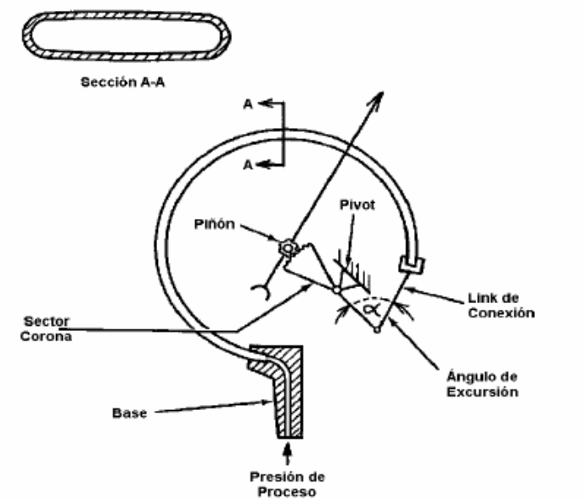
\includegraphics[width=.7\textwidth]{Cap2-DisenoEnsamblado/images/manomBourdon.png}
 \caption{Manómetro de Bourdon, extraído de \cite{bib:ApuntesPuglesiPlacaOrif}}
 \label{fig:manometroBourdon}
\end{figure}

Para conocer los valores de presión en ambas cañerías
(referirse al \gls{pyid}, sección \ref{sec:p&id}),
se instalaron manómetros comunes, de tipo Bourdon\todo{Escala de los manoms?}. 
Un ejemplo de estos manómetros se muestra en la Fig. \ref{fig:manometroBourdon},
donde se observa que un incremento de la presión produce una deformación 
del \emph{tubo de Bourdon}, reflejado en la aguja indicadora.
El manómetro de Bourdon permite obtener una medición visual de la
presión relativa, del punto donde se encuentra instalado.

Durante el montaje, se presentó el problema que uno de los manómetros
no entregaba una medición definida, sino que oscilaba alrededor de un
valor medio (imposibilitando la lectura directa)\todo{por qué pasa esto?}.
Este problema fue solucionado instalando un \textbf{manómetro con glicerina},
donde el mecanismo del manómetro se encuentra sumergido en un baño de glicerina.
Debido a la viscosidad del fluido, las vibraciones quedan amortiguadas
y el manómetro refleja el valor medio de la presión.
